\chapter{Protein Modeling}

\section{Introduction}

Proteins are macromolecules responsible for nearly every task of cellular life. They are 3D structures consisting of amino acid sequences translated from genes and interact with each other to carry out essential functions, such as catalyzing metabolic reaction, transport molecules, respond to stimuli, and so on. Such interactions often happen at sites (e.g. protein domains) that are conserved between proteins across species. By recombining and rearranging these domains as proteins' basic building block, molecular evolution is able to create proteins with different functions.\\

Conventional computational methods for studying protein domains between proteins mainly use the sequences and secondary structures of proteins to do pattern matching, which ignores the 3D nature of proteins and cannot take advantage of the available 3D structures of proteins. For instance, the beginning and the end of an amino acid sequence might come together as a single function group after folding. However, sequential pattern matching would not be able to capture such union. and would produce two separate patterns (one at the beginning and one at the end), instead of a single functional pattern. Therefore, to achieve better understandings about protein interactions and their functions, we need to investigate the detailed spatial characteristics of the 3D structures of proteins. \\

\begin{figure}[h]
	\centering
	\captionsetup{justification=centering}
	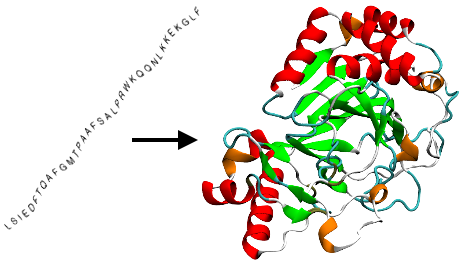
\includegraphics[width=0.7\textwidth]{figs/protein_folding.png}
	\caption[Caption for LOF]{\emph{Conventional computational methods relies sequential data while protein functions in its 3D structure where amino acids that do not appear sequentially could come together to form pattern that are hard to discover in its sequential form.}}
	\label{fig:protein_folding}
\end{figure}

Under such realization, many researchers have started manually matching the 3D structures of proteins, but this is very time consuming and can be subjective. Therefore, if we could generate a good ARG representation for protein 3D structure from crystallography data, our pattern learning could be a great tool for extracting share structure among proteins.

\section{Protein to ARG}

To apply the model on protein crystallography data, we will first need to build a good ARG representation for the protein 3D structure. Protein crystallography data usually comes in as a PDB(Protein Data Bank) format and provides the 3D coordinate $(x, y, z)$ of each amino acid. We turn the 3D structure into a protein ARG where nodes represent different amino acid and edges represent the distance between these amino acids.

\subsection{Edge for Protein ARG}

For the edge protein ARG, we assign it a single scalar which is the euclidian distance of two amino acid:

\begin{equation} 
\overrightarrow{E_{ab}}=\sqrt{(x_a-x_b)^2+(y_a-y_b)^2+(z_a-z_b)^2}
\end{equation}\\

However, we don't want to create an edge for every pair of amino acids. Therefore we choose an $8\AA$ as our distance cutoff, and only create edge for amino acid pairs whose euclidian distance is less than $8\AA$. Here is the histogram for pairwise distance between two amino acids:

\begin{figure}[h]
	\centering
	\captionsetup{justification=centering}
	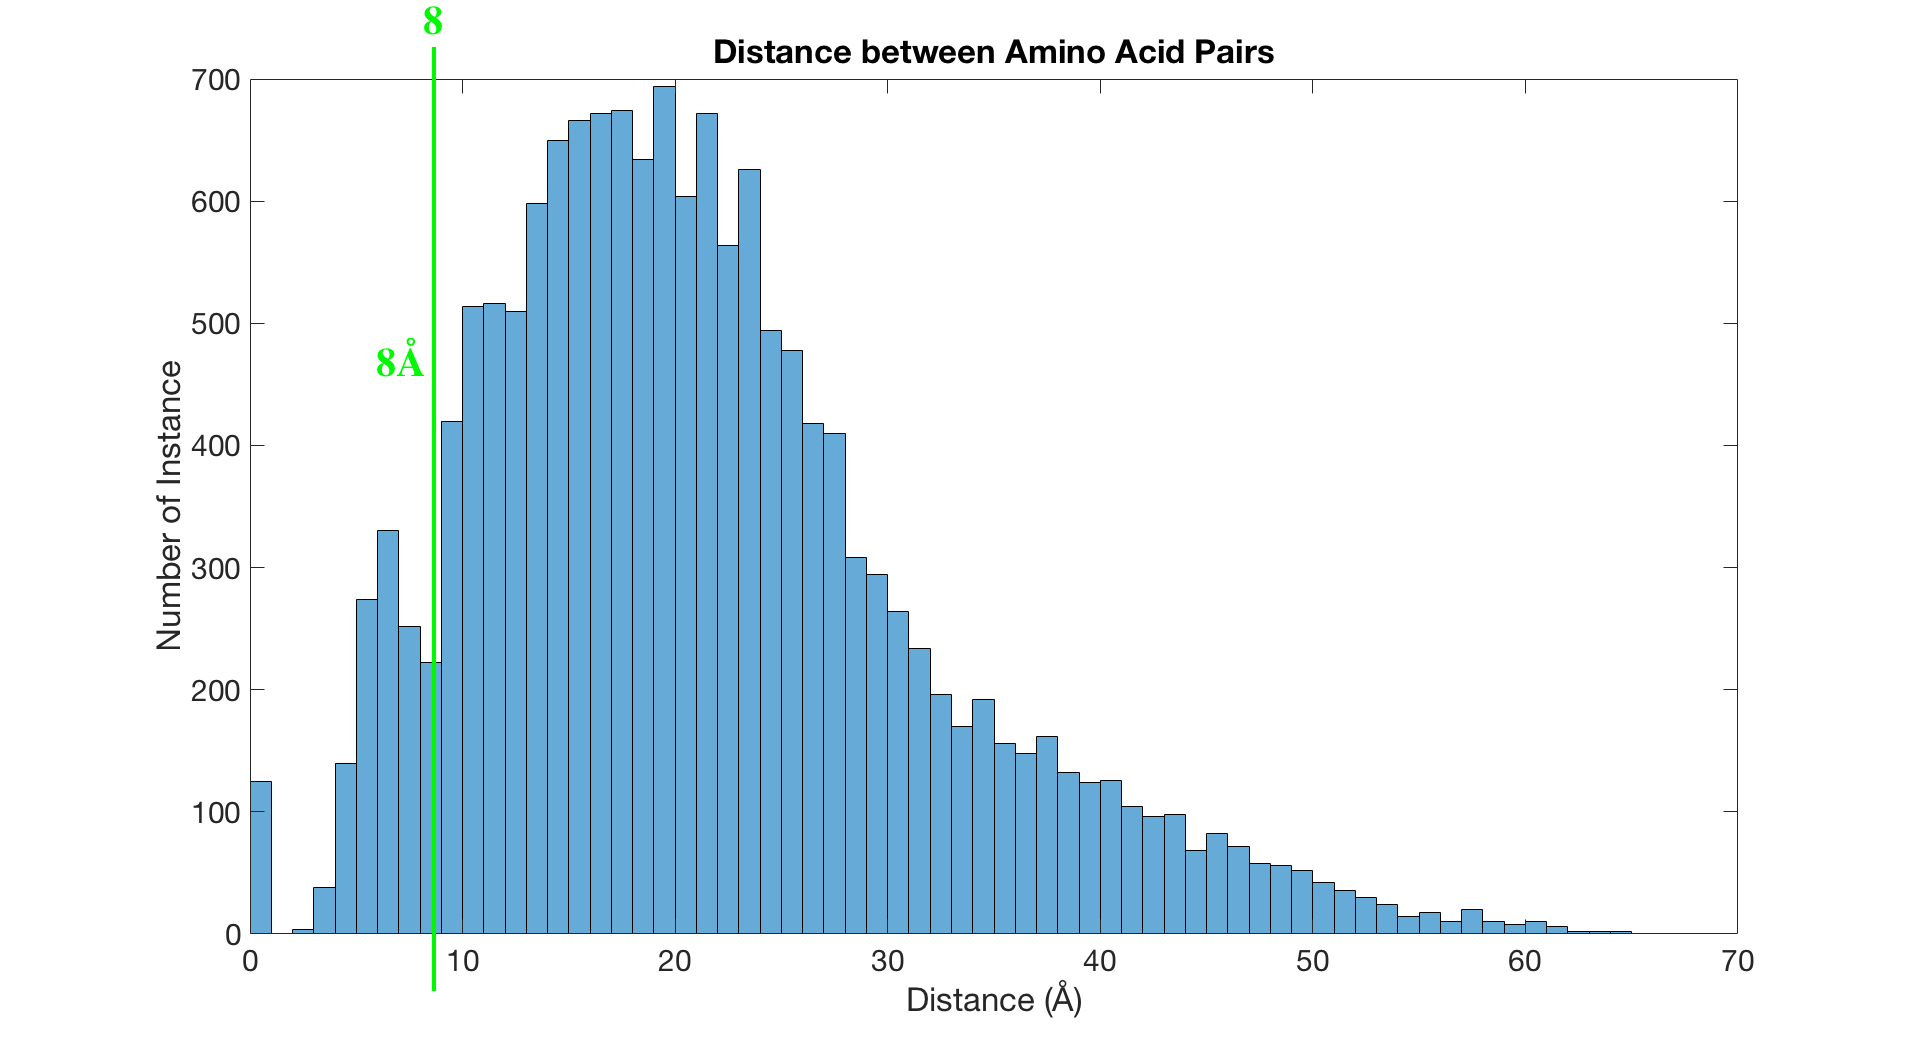
\includegraphics[width=0.9\textwidth]{figs/distance.png}
	\caption[Caption for LOF]{\emph{As expected, we can roughly see a mixture of two normal distribution where the one with the smaller mean representing the distance between two related amino acids while the one with larger mean representing the distance between two random/unrelated amino acids.}}
	\label{fig:distance}
\end{figure}

Interestingly, even though we pick the $8\AA$ cutoff purely based on the distance distribution, a single amino acid also has a diameter $\sim8\AA$.\\

Since $\overrightarrow{E}$ is just a scalar following a normal distribution, we simply used the assume Gaussian PDF to calculate the compatibility and update the mean as well as the variance.

\subsection{Node for Protein ARG}

While setting up the protein ARG edge is pretty straight forward, creating a reasonable representation and compatibility function is very difficult, and here are a couple of options:

\subsubsection{One Hot Representation}
 
The simplest representation for amino acid would just be indexing the $20$ amino acids from $1$ to $20$ and set $\overrightarrow{N}$ to the associated amino acid index. Our compatibility therefore would become:
 
 \begin{equation} 
C_{ai}=\begin{cases}1 & \overrightarrow{N_a}=\overrightarrow{N_i}\\0 & \text{otherwise}\end{cases}
\end{equation}

However, such compatibility function is not biologically accurate because some amino acids might share similar biochemistry property so that they can sometime substitute each other without changing the overall structure of the function unit. Therefore, even though two amino acids have two different name, they can still have some similarity and be compatible in some context. The simple one hot representation in this case does not work.

\subsubsection{BLOSUM Matrix}

Since amino acids that share similar biochemistry property might be compatible in some cases, we also consider using BLOSUM matrix in our compatibility function while keeping the one hot index representation for each node $\overrightarrow{N}$.\\

BLOSUM matrices were first introduced by Steven Henikoff and Jorja Henikoff in 1989. They scanned a protein database with align protein sequence and counted the relative frequencies of amino acids and their substitution probabilities. Then, they calculated a log-odds score and produced a substitution matrix $B$ for the 20 standard amino acids:

\begin{figure}[h]
	\centering
	\captionsetup{justification=centering}
	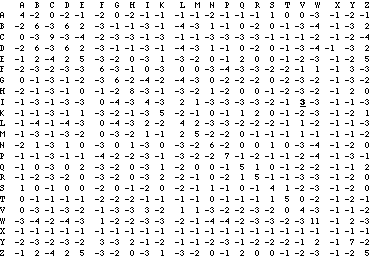
\includegraphics[width=0.7\textwidth]{figs/blosum.png}
	\caption[Caption for LOF]{\emph{Letter here represents different amino acids.}}
	\label{fig:blosum}
\end{figure}

And the compatibility function would then become:

\begin{equation} 
\overrightarrow{C_{ai}}=B[\overrightarrow{N_a},\overrightarrow{N_i}]
\end{equation}

While the BLOSUM matrix $B$ address the problematic compatibility function for one hot representation. Another problem that we would need to address is model node update. If you recall how we update the mean for component node in E.q. \ref{eq:nmean}, we took a weighted average of all the node based on how the node matching probability and sample matching probability. However, since the index is not continuous, it doesn't really make sense to take the mean any more. During our trail, we simply take the index from the node that has the highest weight/matching probability. This is certainly not ideal, and we want to search for a continuous representation for amino acid that are continuous with a compatibility function that consider the similar biochemistry property of different amino acids.

\subsubsection{Amino Acid 2 Vec}
\label{sssec:a2v}

In natural language processing, researchers deal with a similar problem for one hot representation of word. They came up with word embedding based on its surrounding context, and developed a very effective model, Skip-Gram, for generating word vector. With library like Gensim\footnotemark, we can generate our own word vector by simply feeding the model enough document with words.\\
\footnotetext{https://radimrehurek.com/gensim/}

If we think of amino acid sequences as documents and individual amino acid as word, can we generate amino acid vector the same way using model like Gensim? It makes sense because amino acids share similar biochemistry property are likely to stay in a similar chemistry environment created by nearby amino acids. We feed the Skip-Gram model with protein sequences across many species, and get protein vectors $\overrightarrow{AA}$ with a dimension of $20$\footnotemark that cluster by their biochemistry property:
\footnotetext{Since we have 20 amino acids.}

\begin{figure}[h]
	\centering
	\captionsetup{justification=centering}
	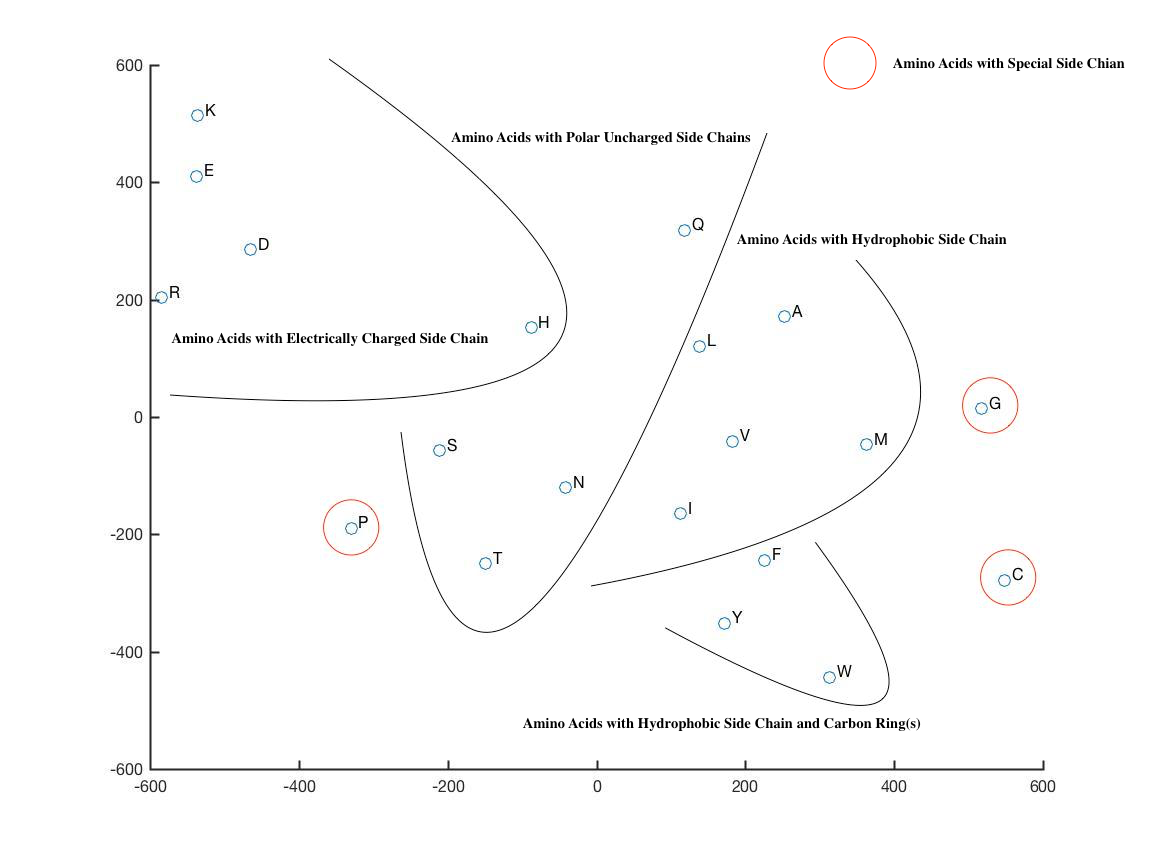
\includegraphics[width=0.9\textwidth]{figs/a2v.png}
	\caption[Caption for LOF]{\emph{Amino Acid Vector $\overrightarrow{AA}$ clusters after dimension reduction (PCA) from $20$ to $2$.}}
	\label{fig:a2v}
\end{figure}

Therefore, we can label each node with its associated amino acid vector and our compatibility function would just be the euclidian distance of the two amino acid vector:

\begin{equation} 
\overrightarrow{C_{ai}}=\sqrt{\sum_{z=1}^{20}(\overrightarrow{N_{a}}[z]-\overrightarrow{N_{i}}[z])^2}
\end{equation}

We also construct a $20\times 20$ compatibility matrix for the $20$ amino acids, and it follow a similar form as the BLOSUM matrix after scaling. For model node, updating mean is  just as easy as follow E.q. \ref{eq:nmean}.\\

This is a very cool idea with lots of potential, but the drawback of such representation would be the lack of locality. Even though our amino acid vector can be clustered by their biochemistry property, they are likely to show slightly different property in different environment, so using a global vector to represent amino acid in different context might not be ideal as well. 

\subsubsection{Local Substitution Vector}

BLOSUM matrix is a brilliant idea as we can calculate the amino acid substitution odd based on protein alignment database. Can we use a similar idea to factor in the locality of the amino acid and solve the model node update problem described above all together?\\

Within the sample protein ARG, each node will have a single amino acid index as their $\overrightarrow{N^s}$. However, for the component protein ARG, the model node $a$ would have a local substitution vector $\overrightarrow{N^w}$ representing the odd for this node to be matched with a specific amino acid. Therefore, the compatibility function would become:

\begin{equation} 
\overrightarrow{C_{ai}^{sw}}=\overrightarrow{N^w_i}[\overrightarrow{N^s_a}]
\end{equation}

Since $\overrightarrow{N^w}$ is continuous substitution vector, we now can easily update the mean for model node update following E.q. \ref{eq:nmean}. But what value should we used for $\overrightarrow{N^w}$, and how should we update it?\\

When initializing the model protein ARG, we set the local substitution vector based on the BLOSUM matrix, so $\overrightarrow{N^w_i}=B[AA_i,:]$, where $AA_i$ is the amino acid index for node $i$. To update the substitution vector with locality, we first calculate a "weighted" frequency vector $\overrightarrow{F^w_i}$:
\begin{align} 
\overrightarrow{\zeta^w_i}[z] = & \sum^{S}_{s=1}\sum^{\{a|\overrightarrow{N^s_a}=z\}}_{a}M^{sw}_{ai}P(G_s=\Phi_w) & \forall z=1,2,3...20\\
\overrightarrow{F^w_i}[z] = & \frac{\overrightarrow{\zeta^w_i}[z]}{\sum^{20}_{x=1}\overrightarrow{\zeta^w_i}[x]} & \forall z=1,2,3...20
\end{align}

Once we calculate $\overrightarrow{F^w_i}$, we can calculate the log odd-ratio with an amino acid background frequency $\overrightarrow{F_B}$ that we can pre-defined or calculate based on the sample protein ARGs:
\begin{align} 
\overrightarrow{N^w_i}[z] = & \text{log}(\frac{\overrightarrow{F^w_i}[z]}{\overrightarrow{F_B}[z]}) & \forall z=1,2,3...20
\end{align}

While this seems complicated, but it is the same idea as BLOSUM matrix. Instead of using a conserve protein alignment database as for BLOSUM, we used our own alignment/matching matrix $M^{sw}$. Since $M^{sw}$ is computed both by amino acid compatibility as well as structure/edge compatibility, we are able to introduced locality into such local substitution vector.

\section{Protein Backbone Encoding in Objective Function}

During the development, we observe matching result where a couple nearby amino acids in one ARG being matched to amino acids that are far apart in another ARG due to similar environment (the first half of E.q. \ref{eq:energy}).\\

However, it's not very likely\footnotemark that three immediate neighbor amino acids in one protein match to entirely different places in another protein. That's because, even though protein can fold, it still has a peptide chain that serve as its backbone that you can't stretch or turn too much. Therefore, we modified the energy/objective function during graph learning E.q. \ref{eq:energy}, and introduced a new term to encode the constraints brought by the protein backbone:
\footnotetext{Though not impossible.}

\begin{align}
E(M)=&-\frac{1}{2}\sum_{a=1}^{G}\sum_{i=1}^{G'}\sum_{b=1}^{G}\sum_{j=1}^{G'}M_{ai}M_{bj}C_{abij}-\alpha\sum_{a=1}^{G}\sum_{i=1}^{G'}M_{ai}C_{ai}\nonumber\\
&\color{red}{-\beta\sum_{a=1}^{G}\sum_{i=1}^{G'}M_{a-1i-1}M_{ai}M_{a+1i+1}}&
\end{align}

While the addition looks complicated, it is simply saying that: if node $a$ in $G$ has a good match with node $i$ in $G'$, than the node immediately before and after node $a$ should also have a good match with the node immediately before and after node $i$ as we are indexing the node by their sequence order.

\section{Proof of Concept}
\label{sec:poc}

Just to do a proof of concept\footnotemark, we trained a model on $5$ protein structure all contains same part of the \emph{CH1} domain with $2$ components and test it on the original structure, mutated structure(reversing the entire sequence, partition the sequence and reverse the order of partition) that are impossible to detect without 3D structure information, and finally random structure:
\footnotetext{Not enough time to do it all!}

\begin{figure}[h]
	\centering
	\captionsetup{justification=centering}
	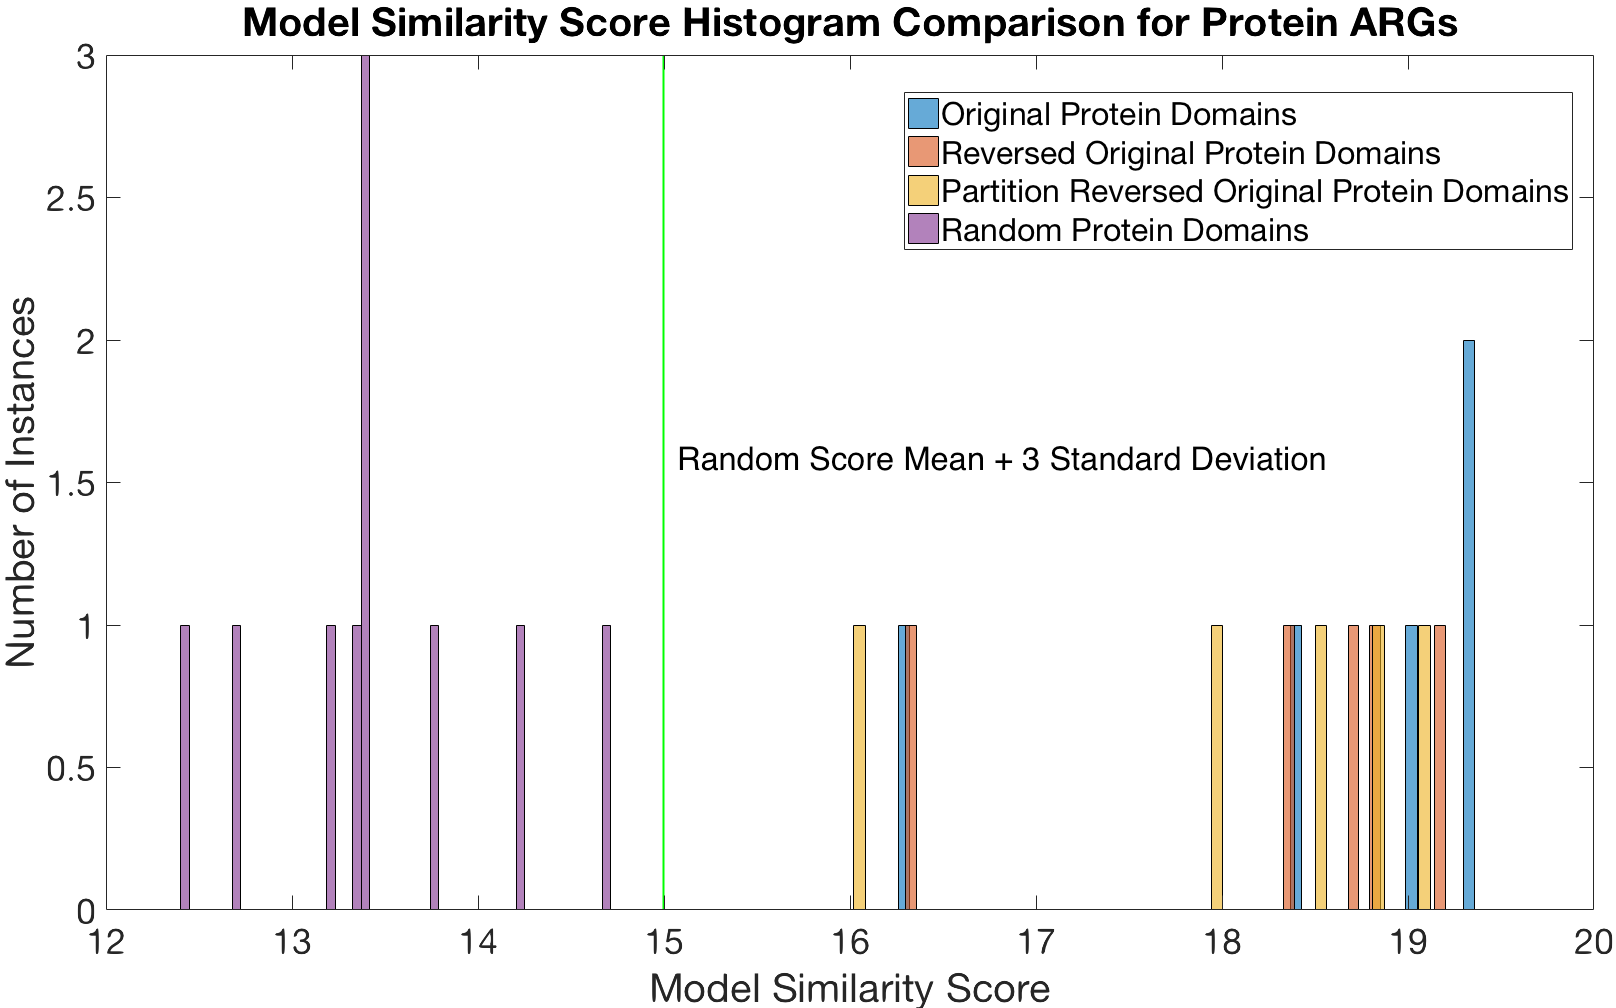
\includegraphics[width=0.79\textwidth]{figs/protein_learning.png}
	\caption[Caption for LOF]{\emph{Model similarity score ($P(G|Z)$) for different test cases.}}
	\label{fig:protein_learning}
\end{figure}

As you can see, our trained model can clearly separate \emph{CH1} domain from random structure. Moreover, for cases where the sequence(indexes) is entirely reversed or reversed in partition (i.e. part of structure move to another place), model are still able to capture the domain. However, if we used traditional sequential matching techniques to find the \emph{CH1} domain, we won't be able to recover the domain if the sequence is reversed or reversed by partition. In addition, our graph matching algorithm also operates in very high precision thanks to the local substitution vector. Here are some examples of protein matching result visualizing in their 3D form:\\

\begin{figure}[h]
	\centering
	\captionsetup{justification=centering}
	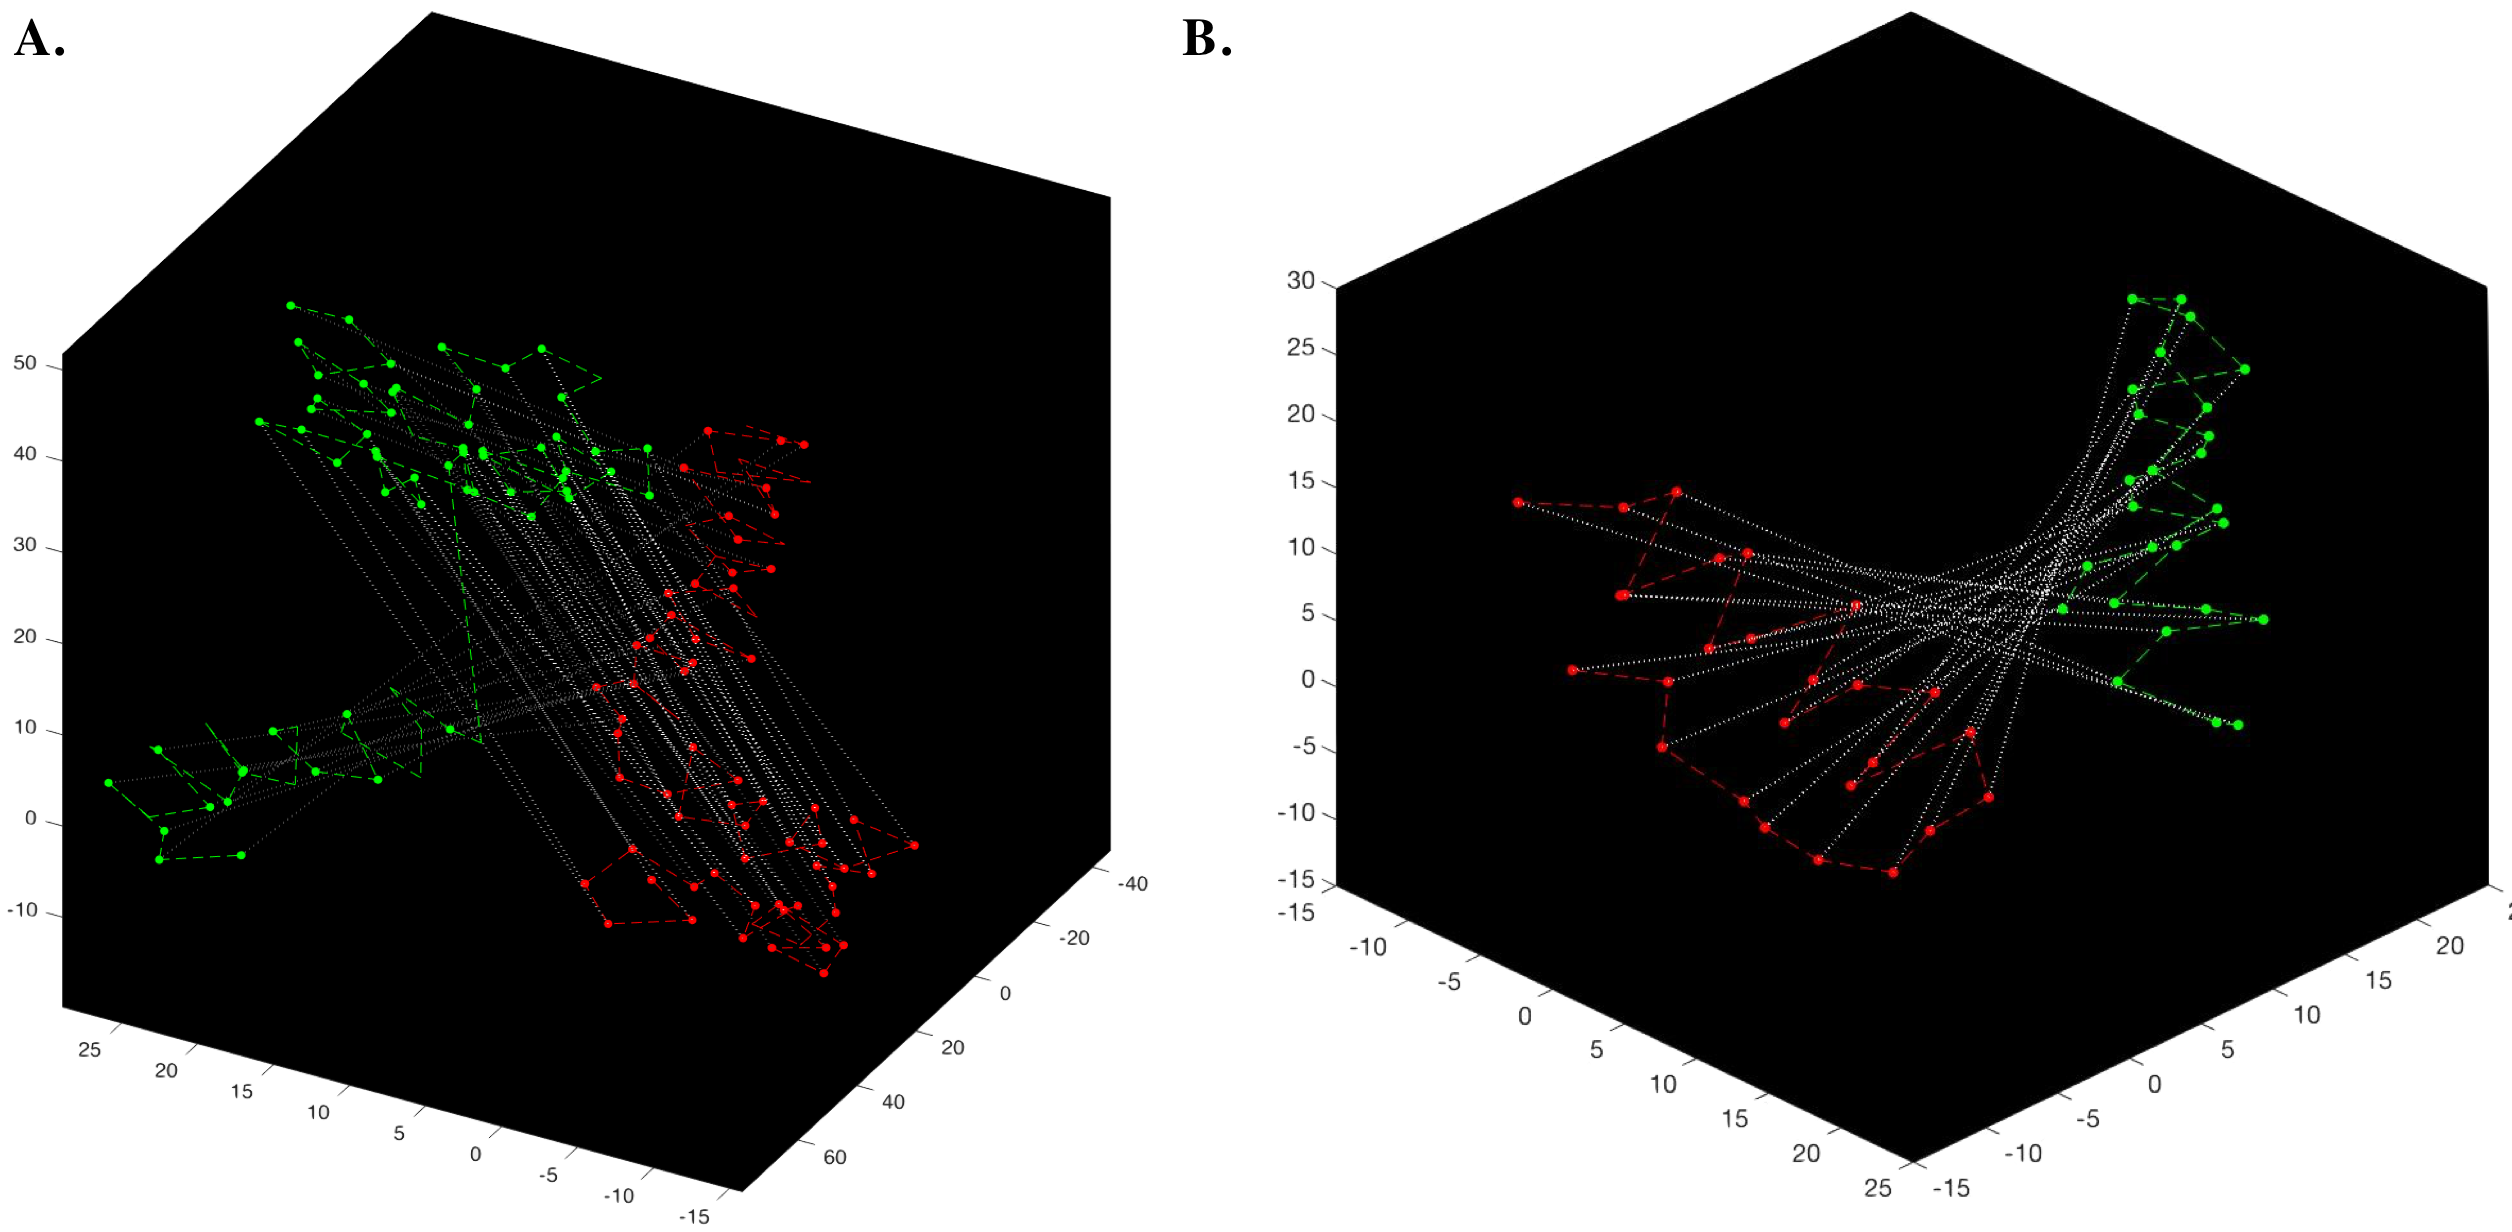
\includegraphics[width=0.95\textwidth]{figs/protein_match.png}
	\caption[Caption for LOF]{\emph{ Two examples of amino acids from two different protein (green and red) are matched (white) based on the graph matching matrix $M$.}}
	\label{fig:protein_match}
\end{figure}


\section{Conclusion}

In this chapter we introduced many ways that we can model the protein 3D structure as a ARG. Then, we show a proof of concept about training a model to learn and summarize part of the \emph{CH1} domain. It shows us how such model can take advantage of the 3D structure data, and recover for sequence changes. Invariance to sequential changes, our model shows potential for discover folded structure and novel motif that are overlooked by traditional sequential alignments.


